% DisagreeBench — arXiv preprint (ACL style, preprint mode)
\documentclass[11pt]{article}
\usepackage[preprint]{acl}
\usepackage{times}
\usepackage{latexsym}
\usepackage[T1]{fontenc}
\usepackage[utf8]{inputenc}
\usepackage{microtype}
\usepackage{graphicx}
\usepackage{booktabs}
\usepackage{amsmath}
\usepackage{amssymb}

\title{Where LLM Annotation Substitutes for Human Labelers --- and Where It Doesn't:\\ Uncertainty Channels and the Economics of Routing Contested Items}

\author{Yogya Mehrotra \\
  \texttt{yogyamehrotra@gmail.com} \\
  \texttt{github.com/yogyam/DisagreeBench}}

\begin{document}
\maketitle

\begin{abstract}
The case for replacing human annotators with LLMs typically rests on a single aggregate agreement number. We test the hypothesis that this number is structurally misleading: that LLM--human agreement is high exactly where humans already agree with each other, and collapses where they don't. Using ChaosNLI (3,113 SNLI/MNLI items with 100 human annotations each), we elicit a label \emph{distribution} from claude-sonnet-5 via self-consistency sampling (10 samples per item) and compare it to the human distribution with Jensen--Shannon divergence (JSD), stratified by human label entropy. The hypothesis holds: mean JSD rises monotonically from 0.07 [95\% CI 0.06, 0.09] in the lowest-entropy quintile to 0.31 [0.30, 0.32] in the highest, while the conventional metric --- accuracy against the majority label --- declines far more gently ($0.94 \rightarrow 0.56$) and therefore flatters the model precisely on the contested items. We then test whether the model's own uncertainty could route hard items to humans, and find it cannot: the model is fully deterministic across its 10 samples on 85\% of items --- including most items where humans split near 50/50 --- and the rank correlation between model self-consistency entropy and human entropy is $\rho = 0.164$ [0.131, 0.196], decisively below any usefully routable signal; enabling reasoning does not change this. The contrast is stark: the human pool's inter-annotator agreement is Krippendorff's $\alpha = 0.37$; the model's agreement with itself is $\alpha = 0.90$. Yet when asked to \emph{estimate} the annotator distribution directly, the same model produces distributions $3\times$ closer to the human ones (JSD 0.07) whose entropy does clear the routing threshold ($\rho = 0.393$). The model's behavioral uncertainty carries no information about human disagreement --- but its declarative estimate of human disagreement does. Finally, we run the budget-allocation experiment this signal enables: a simulated router that sends the top-scoring items to $k$ human annotators and keeps the model's distribution for the rest. Against the realistic baseline (model self-consistency distributions), routing on verbalized entropy captures 37\% of an expected-gain oracle's achievable improvement, and random allocation needs ${\sim}1.5\times$ the annotation budget to match it. Against the strongest baseline (the model's own verbalized distributions), the same signal is \emph{worse than random}: the model's residual errors hide in items it is confidently wrong about. Model-reported uncertainty tells you where the task is hard --- not where the model is wrong.
\end{abstract}

\section{Motivation}
\label{sec:motivation}

Data-labeling providers are being asked to justify themselves against claims of the form ``the model agrees with human labels 90\% of the time at 1\% of the cost.'' That figure is an average over a distribution of examples that is sharply bimodal in difficulty: most items in a real annotation stream are unambiguous, while a minority are genuinely contested --- and the contested minority consumes most of a real annotation budget and drives most disagreement in downstream training. If LLM agreement concentrates on the easy majority, a headline agreement figure can be technically true and operationally misleading, and the correct architecture is neither ``replace humans'' nor ``keep humans'' but \emph{triage}. This study measures the premise of that argument directly, and then tests whether the triage router is buildable from the model's own uncertainty.

\section{Data}
\label{sec:data}

\textbf{ChaosNLI} \citep{nie2020chaosnli} provides ${\sim}100$ annotations per item for 4,645 development-set items from SNLI, MNLI, and Abductive NLI. We use the SNLI (1,514) and MNLI (1,599) portions --- 3,113 items sharing the 3-way entailment/neutral/contradiction label space --- and exclude Abductive NLI (a 2-way task). The 100-annotator sample gives a genuine label distribution per item rather than a noisy 3--5-rater estimate, which is what makes entropy stratification statistically meaningful. Items are bucketed into quintiles of human label entropy computed from the full distribution (quintile edges: 0.66, 0.91, 1.05, 1.21 bits).

The pool is genuinely contested: nominal Krippendorff's $\alpha$ is 0.447 (SNLI), 0.283 (MNLI), 0.367 combined. This is by construction --- ChaosNLI drew items whose original 5-rater annotations disagreed --- and it is exactly the regime the substitution argument is quietly averaged over.

\section{Method}
\label{sec:method}

\paragraph{Elicitation.} claude-sonnet-5 (Anthropic), accessed via the Message Batches API. Each item is sampled 10 times as an independent request. The label options are presented in randomized order per sample (mitigating option-ordering bias); output is constrained to a JSON schema over the three labels, so every sample parses; extended thinking is disabled. The empirical distribution over the 10 sampled labels is the model's label distribution. Of 31,130 requests, 31,127 returned usable labels (3 errors).

\paragraph{Verbalized arm.} As a comparison elicitation (one request per item, full 3,113-item set), the model is asked to estimate how 100 careful annotators would distribute over the three labels, output as integer percentages under the same schema constraint.

\paragraph{Router simulation.} Each item's 100 annotations are split 50/50: one half defines the ground-truth distribution, the other is the finite pool routed items draw from (so the router can never ``buy'' the evaluation target, and even perfect routing pays annotator-sampling noise). A router scores all items, sends the top fraction $f$ to humans --- receiving $k$ annotations drawn without replacement from the pool --- and keeps the model's distribution for the rest. We sweep $f$ from 0 to 1 and $k \in \{1, 3, 5, 10, 20, 50\}$, with 20 replicate splits. Strategies: random; self-consistency entropy; verbalized entropy; channel disagreement (JSD between the sampled and verbalized distributions); an \emph{entropy oracle} scoring by true human entropy; and two regret oracles scoring by each item's actual improvement from routing --- \emph{expected gain} (Monte-Carlo mean over 200 redraws; the fair upper bound, since it knows which items benefit but not the luck of the draw) and \emph{realized gain} (a skyline that peeks at the draw). Headline numbers: AUC of the budget--JSD curve, normalized as the share of the expected-gain oracle's improvement over random (``capture''); and budget-to-match, the multiple of annotations random allocation needs to reach a strategy's JSD at a given budget. Item-level bootstrap (1,000 resamples) gives CIs on strategy--random gaps. Everything is repeated with total variation distance in place of JSD and with a bootstrap-resampling split protocol in place of the 50/50 split.

\paragraph{Metrics.} Primary: per-item Jensen--Shannon divergence (base 2) between the model and human label distributions, averaged per entropy quintile. Reported alongside, explicitly as the metric under critique: accuracy of the model's modal label against the human majority label. The routing gate: Spearman rank correlation between model self-consistency entropy and human entropy. All means and the correlation carry 95\% percentile bootstrap CIs (10,000 resamples). Contamination diagnostic: agreement of the modal label with the \emph{original} single gold label vs.\ with the ChaosNLI majority, per quintile.

\section{Results}
\label{sec:results}

\subsection{Agreement degrades with human disagreement --- and accuracy hides it}
\label{sec:stratified}

\begin{table}[t]
\centering
\small
\begin{tabular}{lccc}
\toprule
Quintile & $n$ & Mean JSD [CI] & Acc.\ vs.\ maj.\ [CI] \\
\midrule
Q1 (low) & 631 & 0.074 [.064, .085] & 0.945 [.926, .962] \\
Q2 & 615 & 0.178 [.165, .192] & 0.805 [.772, .836] \\
Q3 & 623 & 0.244 [.232, .255] & 0.674 [.637, .711] \\
Q4 & 622 & 0.263 [.254, .273] & 0.614 [.576, .653] \\
Q5 (high) & 622 & 0.311 [.302, .321] & 0.558 [.519, .596] \\
\bottomrule
\end{tabular}
\caption{Model--human divergence and accuracy against the majority label, by quintile of human label entropy (95\% bootstrap CIs).}
\label{tab:stratified}
\end{table}

\begin{figure}[t]
\centering
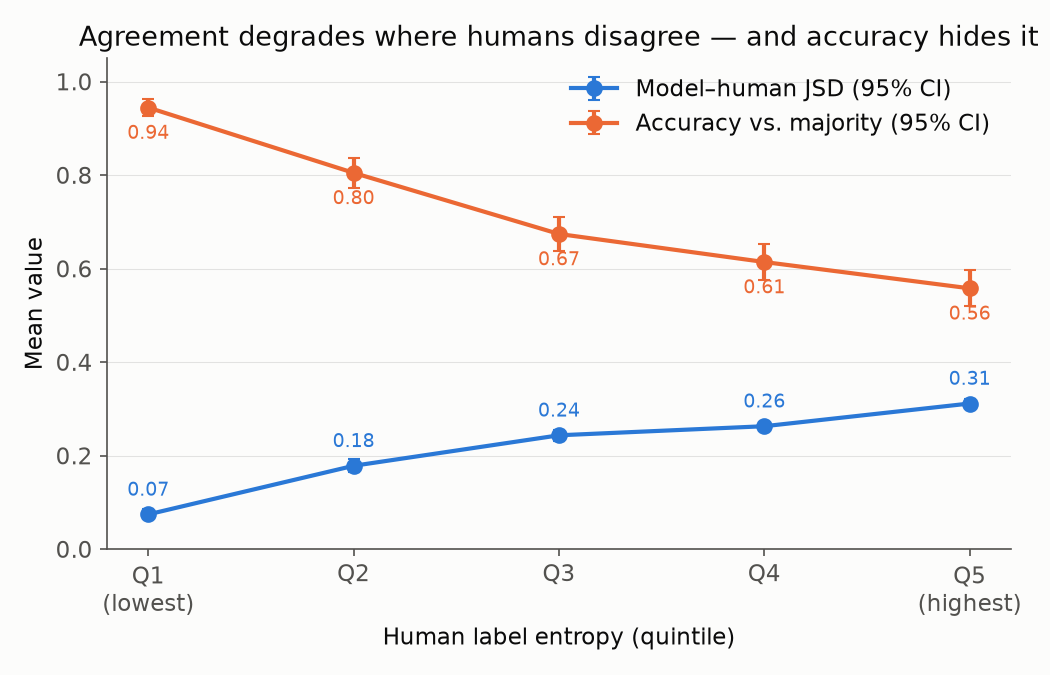
\includegraphics[width=\columnwidth]{figures/jsd_vs_entropy_examples.png}
\caption{Mean JSD between model and human label distributions (blue) and accuracy against the majority label (orange) across human-entropy quintiles. The divergence quadruples while accuracy declines gently: the standard metric is most flattering exactly where the model is furthest from the human distribution.}
\label{fig:stratified}
\end{figure}

JSD rises monotonically by a factor of ${\sim}4.2$ from Q1 to Q5 (Table~\ref{tab:stratified}, Figure~\ref{fig:stratified}). This deliberately replicates the stratified diagnostic \citet{nie2020chaosnli} ran on fine-tuned encoders, and the shape has changed in a way that matters: where their models' accuracy fell to chance on contested items, the frontier LLM stays well above it, and its Q1 JSD now reaches their estimated human bound (${\sim}0.06$). Accuracy against the majority declines much more slowly, and its floor is deceptive: on Q5 items the human majority is itself close to a coin flip, so ``56\% accuracy'' largely reflects picking the more common side of a split --- not agreement with what humans collectively believe. The gap between the two curves is the headline finding: \textbf{the standard metric is most flattering exactly where the model is furthest from the human distribution.}

\subsection{The gate fails: model uncertainty is not human uncertainty}
\label{sec:gate}

\begin{figure}[t]
\centering
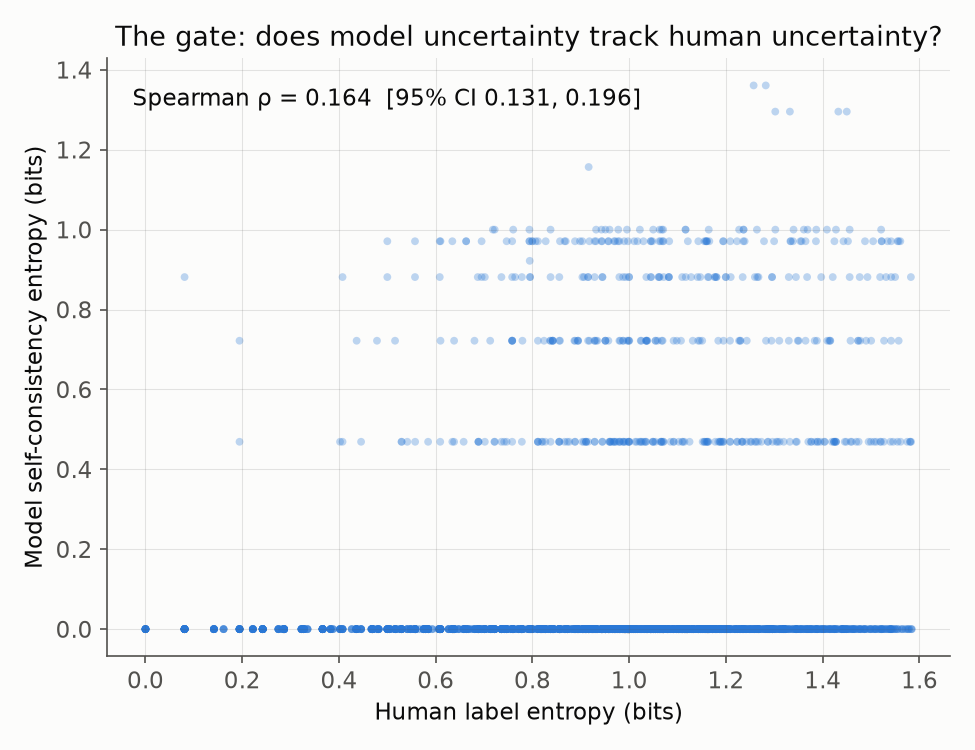
\includegraphics[width=\columnwidth]{figures/gate_scatter_examples.png}
\caption{Model self-consistency entropy vs.\ human label entropy. The model sits at zero entropy on 85\% of items regardless of how contested they are; $\rho = 0.164$.}
\label{fig:gate}
\end{figure}

If a model knew which items humans find hard, its uncertainty could route those items to people. It does not. Across 10 samples the model returns the identical label on 2,653 / 3,113 items (85\%) --- including 84\% of Q5, where human annotators split at more than 1.2 bits of entropy. Where the human pool agrees at $\alpha = 0.367$, the model agrees with itself at $\alpha = 0.904$.

The rank correlation between model self-consistency entropy and human entropy is $\rho = 0.164$ [95\% CI 0.131, 0.196] ($p \approx 4\times10^{-20}$; Figure~\ref{fig:gate}). The correlation is reliably nonzero --- the model is not blind to difficulty --- but the CI excludes by a wide margin any threshold ($\geq{\sim}0.3$) at which uncertainty-based routing would meaningfully beat random allocation. An ablation with adaptive thinking enabled (\S\ref{sec:limitations}) leaves the picture unchanged. By the pre-registered logic of the study design, self-consistency entropy is disqualified as a router input: \textbf{this routing signal does not exist} (\S\ref{sec:router} confirms end-to-end that routing on it is no better than random). The signal that does exist comes from a different channel entirely (\S\ref{sec:verbalized}).

\subsection{Verbalized confidence: the model can report disagreement it does not enact}
\label{sec:verbalized}

Prompted instead to \emph{estimate} the human distribution directly --- ``imagine 100 careful annotators; how many choose each label?'' (one request per item) --- the model behaves entirely differently (Table~\ref{tab:verbalized}).

\begin{table}[t]
\centering
\small
\setlength{\tabcolsep}{4pt}
\begin{tabular}{lccc}
\toprule
Signal & JSD & Entropy (bits) & Gate $\rho$ \\
\midrule
Sampled ($10\times$) & 0.224 & 0.089 & 0.164 \\
Verbalized & \textbf{0.072} & \textbf{0.863} & \textbf{0.393} \\
Human pool & --- & 0.939 & --- \\
\bottomrule
\end{tabular}
\caption{Mean JSD vs.\ the human distribution, mean entropy, and Spearman correlation with human entropy, for the two elicitation channels (full set, $n = 3{,}113$; verbalized gate $p \approx 10^{-113}$).}
\label{tab:verbalized}
\end{table}

Verbalized distributions are ${\sim}3\times$ closer to the human distribution than sampled ones, their average entropy nearly matches the human pool's, and verbalized entropy clears the pre-registered routing threshold ($\rho = 0.393 \geq 0.3$; pilot estimate was 0.354). Where sampled JSD degrades $4.2\times$ from the lowest- to highest-entropy quintile (\S\ref{sec:stratified}), verbalized JSD is nearly flat: $0.044 \rightarrow 0.103$. The declarative estimate stays accurate on precisely the contested items where the behavioral distribution collapses. Strikingly, the two uncertainty signals are essentially uncorrelated with each other ($\rho = 0.03$--$0.08$, depending on which sampled run is paired): they measure different quantities. Together with \S\ref{sec:gate}, this yields the paper's sharpest formulation: \textbf{the model's \emph{behavioral} uncertainty carries no information about human disagreement, but its \emph{declarative} estimate of human disagreement does.} This inverts a common assumption (including in our own study design) that verbalized probabilities are poorly calibrated and self-consistency is the trustworthy signal. It also conditionally revives the triage router: the routing signal exists --- it just has to be asked for, not observed.

The direction of this contrast --- verbalized beats sampled, and reasoning does not close the gap --- independently replicates what \citet{ni2026reasoning} report on hate-speech, emotion, and preference tasks and \citet{meister2025benchmarking} on opinion surveys; \S\ref{sec:related-channels} details what is new here (the entropy-flatness, the channel independence, and the routing consequences in \S\ref{sec:router}).

One caveat attaches specifically to this result: ChaosNLI's label \emph{distributions} have been public since 2020 --- and are by now an explicit optimization target in the literature \citep[e.g.,][fine-tunes directly on them]{wu2026shala} --- so the model may have absorbed some of them in pretraining. A memorized distribution would inflate verbalized performance in a way the gold-label diagnostic in \S\ref{sec:contamination} does not cover. Replication on held-out or post-cutoff annotation data is required before the verbalized result is load-bearing.

\subsection{The result is not memorization}
\label{sec:contamination}

ChaosNLI is built on SNLI/MNLI, which are almost certainly in the model's pretraining data; a model could look good by reciting original gold labels. The diagnostic says otherwise: the modal label agrees with the ChaosNLI majority \emph{more} than with the original gold label in Q1--Q3 (e.g.\ 0.945 vs.\ 0.857 in Q1), and the two converge in Q4--Q5 (0.614 vs.\ 0.637; 0.558 vs.\ 0.539). If the model were reproducing memorized gold labels, the pattern would invert on high-entropy items, where the original gold is essentially arbitrary. It does not (Figure~\ref{fig:contamination}).

\begin{figure}[t]
\centering
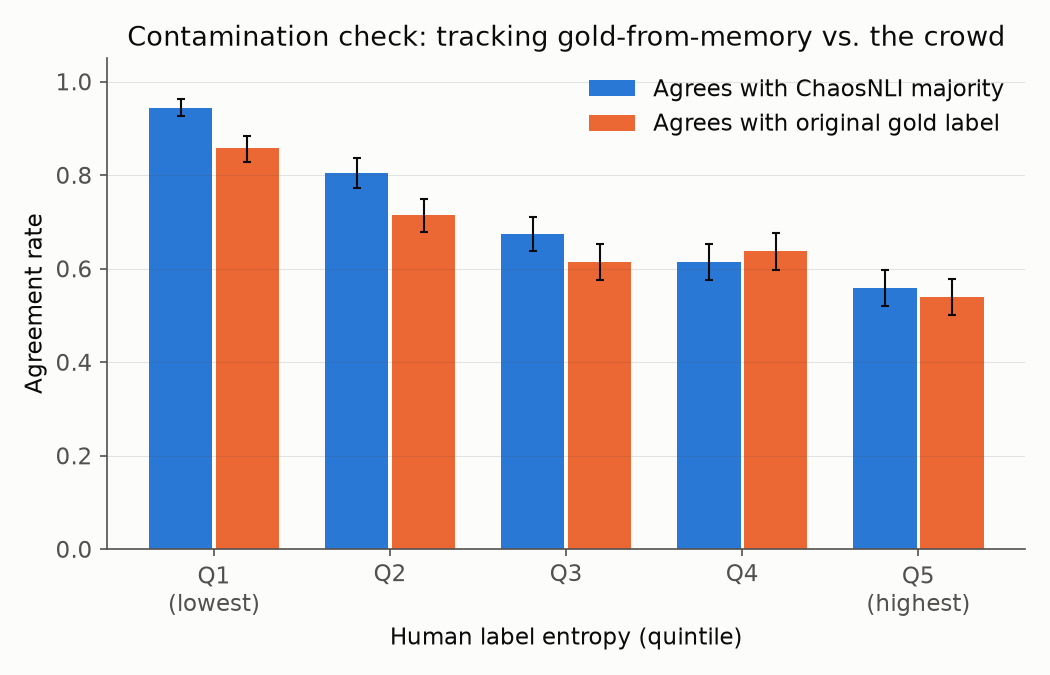
\includegraphics[width=\columnwidth]{figures/contamination_examples.png}
\caption{Modal-label agreement with the ChaosNLI 100-annotator majority vs.\ the original single gold label, by quintile. The model tracks the crowd, not the memorized gold.}
\label{fig:contamination}
\end{figure}

\subsection{The router: uncertainty finds hard items, not model errors}
\label{sec:router}

The simulation (method in \S\ref{sec:method}) asks the operational question directly: given a fixed annotation budget, does routing on model-reported uncertainty beat spending the same budget at random? The answer splits cleanly by what the unrouted items fall back to.

\begin{figure*}[t]
\centering
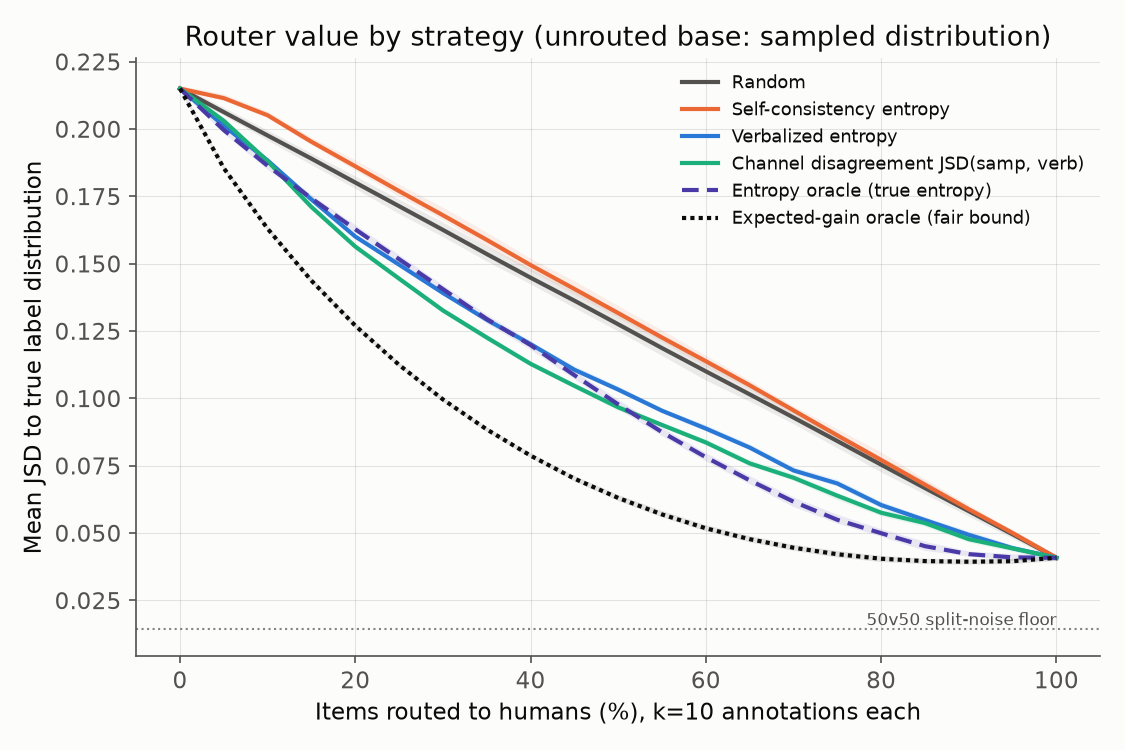
\includegraphics[width=0.49\textwidth]{figures/router_sampled_examples.png}\hfill
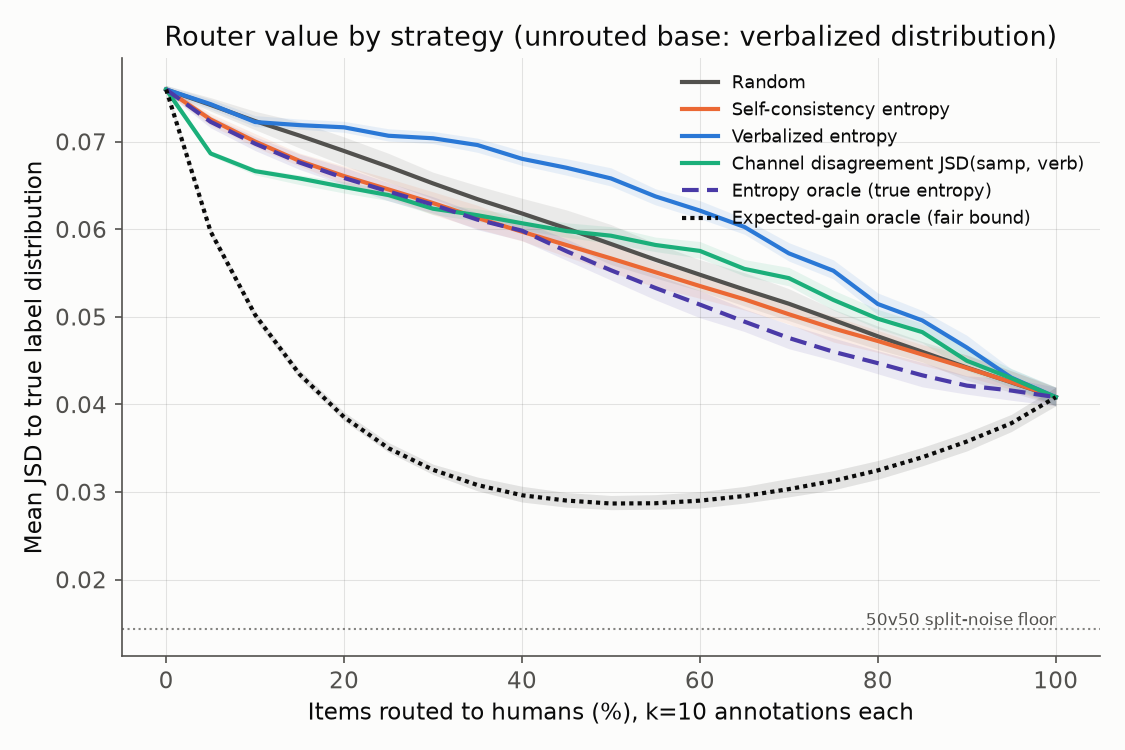
\includegraphics[width=0.49\textwidth]{figures/router_verb_examples.png}
\caption{Router value curves at $k = 10$ annotations per routed item. \textbf{Left:} unrouted items keep the model's sampled distribution --- verbalized-entropy and channel-disagreement routing approach the true-human-entropy oracle. \textbf{Right:} unrouted items keep the model's verbalized distribution --- the same verbalized-entropy signal is now \emph{worse than random} (anti-selection), and even the true-entropy oracle barely beats random; the expected-gain oracle shows the errors remain findable in principle.}
\label{fig:router}
\end{figure*}

\paragraph{Against the sampled base} --- the realistic setting where un-routed items keep the model's self-consistency distribution --- verbalized-entropy routing works (Figure~\ref{fig:router}, left). At $k = 10$ annotations per routed item it captures \textbf{37.4\%} of the expected-gain oracle's improvement over random; channel disagreement (JSD between the model's two distributions, using no human information) captures \textbf{45.5\%}, statistically indistinguishable from the \emph{true-human-entropy} oracle (47.7\%). In budget terms, random allocation needs \textbf{1.44--1.57$\times$} as many annotations to match verbalized-entropy routing at 10--30\% coverage (strategy--random gap CIs exclude zero at every budget above 5\%). Self-consistency entropy captures nothing ($-8.3$\%), closing the loop on \S\ref{sec:gate} with an end-to-end null.

\paragraph{Against the verbalized base} --- where un-routed items keep the model's verbalized distribution, the stronger baseline \S\ref{sec:verbalized} establishes --- the same signal \emph{inverts} (Figure~\ref{fig:router}, right): verbalized entropy is reliably worse than random (capture $-18.7$\%; random matches it with 0.5--0.6$\times$ the budget). The mechanism is anti-selection. High verbalized entropy flags items where humans genuinely disagree --- but \S\ref{sec:verbalized} showed the verbalized distribution is already accurate exactly there. The residual errors sit in low-entropy items the model is confidently wrong about, which entropy routing systematically deprioritizes (per-item verbalized entropy vs.\ verbalized error: $\rho \approx -0.07$). Even the true-human-entropy oracle barely beats random here (11.9\%), while the expected-gain oracle still improves substantially --- the errors are findable in principle, just not by any entropy-shaped signal. \textbf{Model-reported uncertainty tells you where the task is hard, not where the model is wrong}; it routes usefully only when the fallback annotator is weak.

\begin{figure*}[t]
\centering
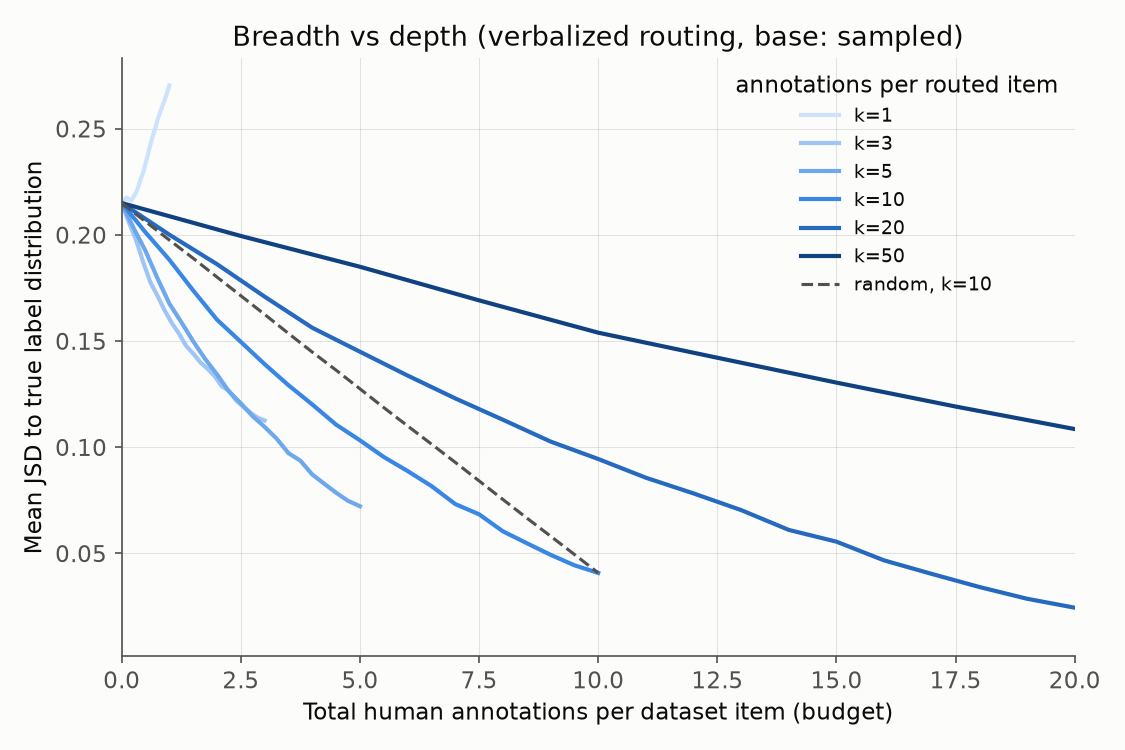
\includegraphics[width=0.49\textwidth]{figures/router_ksweep_sampled_examples.png}\hfill
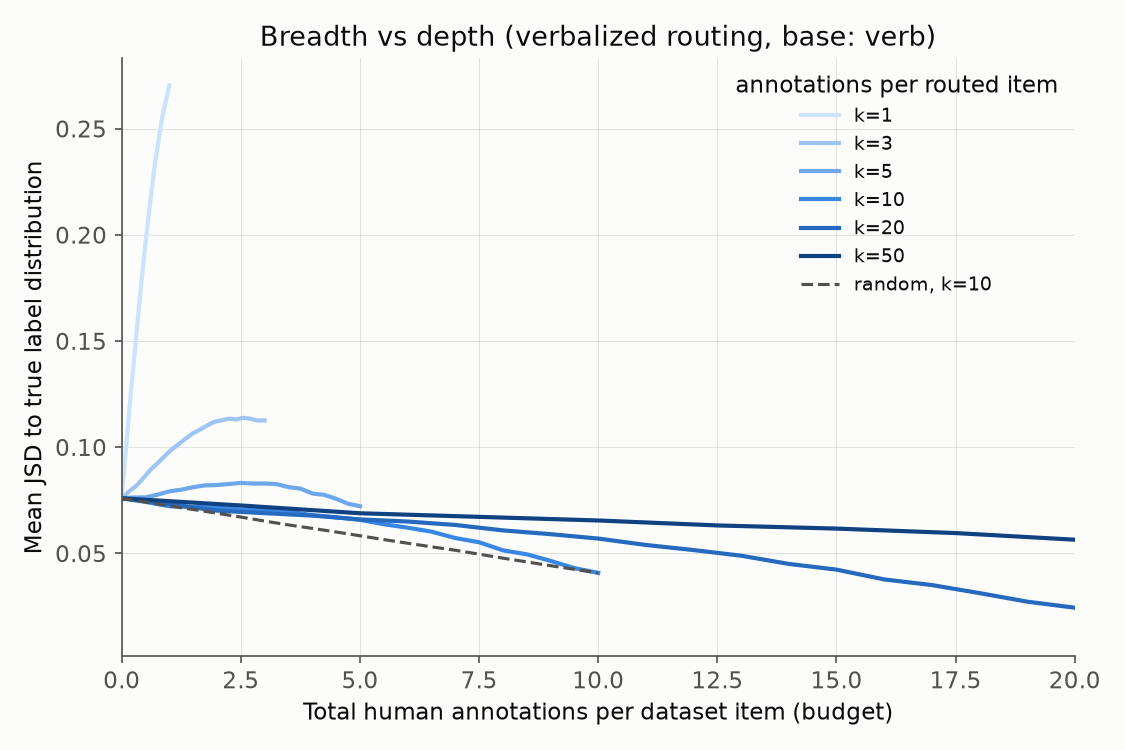
\includegraphics[width=0.49\textwidth]{figures/router_ksweep_verb_examples.png}
\caption{Breadth vs.\ depth: value of verbalized-entropy routing as a function of total annotation budget, for different annotation depths $k$ per routed item. \textbf{Left:} sampled base --- shallow-and-broad ($k = 3$--$5$) dominates deep-and-narrow. \textbf{Right:} verbalized base --- replacing the model's verbalized distribution with the empirical distribution of $k$ human labels only breaks even at $k \approx 5$; at $k = 1$ routing makes the corpus estimate strictly worse.}
\label{fig:ksweep}
\end{figure*}

\paragraph{Breadth vs.\ depth.} Sweeping $k$ (Figure~\ref{fig:ksweep}) shows that at a fixed total budget, shallow-and-broad beats deep-and-narrow on the sampled base ($k = 3$--$5$ dominates $k = 20$--$50$), and yields the study's most quotable number on the verbalized base: replacing the model's verbalized distribution with the empirical distribution of $k$ human labels only breaks even at $k \approx 5$ ($k = 1$: JSD 0.270; $k = 3$: 0.113; $k = 5$: 0.072; model verbalized: 0.076). In distributional terms, one model call is worth roughly five human annotations on this dataset --- with the memorization caveat of \S\ref{sec:verbalized} attached.

All orderings and magnitudes are stable under total variation distance in place of JSD and under the bootstrap split protocol (capture 37.7--38.9\% verbalized, 44.0--46.8\% channel disagreement on the sampled base; anti-selection persists on the verbalized base in every variant).

\section{Related Work}
\label{sec:related}

\subsection{Human label variation and distributional evaluation}
\label{sec:related-hlv}

That disagreement in NLI judgments is reproducible signal rather than annotation noise was established by \citet{pavlick2019inherent}, and the position that label variation should be modeled rather than adjudicated away is now a program \citep{plank2022problem,uma2021learning,basile2021weneed,cabitza2023perspectivist}. Our evaluation toolkit is theirs: JSD against the human label distribution and the correlation between per-item model and crowd entropy are both standardized in \citet{uma2021learning}. Our dataset paper, ChaosNLI \citep{nie2020chaosnli}, already performed the stratified analysis for fine-tuned encoders: accuracy degrades toward chance and JSD stays above 0.2 as human agreement falls. \S\ref{sec:stratified} is a deliberate replication of that diagnostic on a frontier LLM, and what changed is the shape: the model now reaches the estimated human JSD bound (${\sim}0.06$) on high-agreement items, and accuracy on contested items no longer collapses to chance (0.56 vs.\ 0.33) --- which makes the flattery problem \emph{worse}, because the standard metric now looks respectable everywhere while distributional divergence quadruples. Distributed NLI \citep{zhou2022distributed} formalized the task of predicting human opinion distributions on ChaosNLI: their supervised estimators (MC Dropout, recalibration, distillation) reach JSD $\approx 0.18$--$0.19$, which our zero-supervision verbalized elicitation beats by ${\sim}2.5\times$; their appendix also documents that encoder uncertainty is miscalibrated against human disagreement, a precursor of our gate analysis. \citet{baan2022stop} showed on ChaosNLI that calibration to a majority label is incoherent under disagreement (our 50/50 truth/pool split in \S\ref{sec:method} adapts their device of splitting the 100 annotations into sub-populations); \citet{baan2024interpreting} argue conceptually that a predictive distribution conflates model confidence with human variation --- our channel-decorrelation finding (\S\ref{sec:verbalized}) turns that distinction into a measured property. VariErr NLI \citep{webergenzel2024varierr} implies some of ChaosNLI's variation is annotation error, which makes our router's measured gains conservative with respect to error-cleaned targets.

\subsection{LLMs as annotators}
\label{sec:related-annotators}

The replacement wave \citep{gilardi2023chatgpt,tornberg2023chatgpt} reads the model's high self-consistency as annotation quality; on contested items we show the same property is a liability --- the model agrees with itself ($\alpha = 0.90$) about questions on which 100 humans split nearly evenly ($\alpha = 0.37$). \citet{reiss2023testing} complained that 2023-era ChatGPT was too \emph{unstable} to annotate reliably; 2026 frontier models exhibit the opposite pathology, and neither regime tracks human disagreement. \citet{baumann2025hacking} quantify the downstream stakes --- LLM annotation choices flip roughly a third of tested conclusions --- and already propose verbalized-confidence-targeted human annotation as a mitigation, evaluated against disagreement-filtered gold labels; our anti-selection result (\S\ref{sec:router}) exposes a failure mode of exactly that strategy once the target is the label distribution and the fallback is the model's own best output.

\subsection{LLM uncertainty channels and human disagreement}
\label{sec:related-channels}

\citet{lee2023dissenting} first compared sampled and logprob-derived LLM distributions to ChaosNLI's annotator distributions, observing that GPT-3's output entropy is near zero and visibly uncorrelated with human entropy. Our \S\ref{sec:gate} quantifies that observation at frontier scale (85\% exact determinism; $\alpha = 0.90$ vs.\ 0.37; gate $\rho = 0.164$ with CIs) and stress-tests it against reasoning and paraphrase confounds. \citet{madaan2025lost} stratify accuracy by human entropy for open-weight models on ChaosNLI; the accuracy/JSD \emph{dissociation} across quintiles is ours. The channel contrast we find was anticipated on other tasks: \citet{ni2026reasoning} show verbalized distributions beat sampled ones for disagreement prediction on hate-speech, emotion, and preference tasks (and that RLVR-style reasoning hurts); \citet{meister2025benchmarking} found LLMs describe opinion distributions better than they simulate them; \citet{jang2026instruction} attribute the simulation failure to alignment-induced mode collapse \citep[cf.][]{kirk2024understanding}, consistent with the calibration literature where asking beats token probabilities \citep{lin2022teaching,tian2023just,kadavath2022language} --- though against \emph{correctness}, consistency-based signals often win \citep{xiong2024can}, underlining that our target is different. \citet{wang2024myanswer} show first-token probabilities diverge from what instruction-tuned models actually answer, which is why we omit a logprob arm. On NLI specifically, \citet{chen2024seeing,chen2025rose} approximate human judgment distributions with explanation-conditioned LLM prompting, and \citet{chen2026decoupling} show CoT does not calibrate distributions on ambiguous items. Relative to all of these, our \S\ref{sec:verbalized}--\ref{sec:contamination} contribute: replication of the verbalized--sampled gap on 100-way NLI distributions with a frontier model; the near-flatness of verbalized JSD across disagreement levels; the statistical \emph{independence} of the two channels' entropies ($\rho \leq 0.08$), which no prior work reports; and the gate framing that connects channel quality to routability. \citet{zhang2025verbalized} propose verbalized sampling to recover output diversity; our results externally validate the verbal channel against ground-truth human distributions rather than diversity alone.

\subsection{Hybrid annotation and budget allocation}
\label{sec:related-routing}

Routing between model and human annotators instantiates learning-to-defer \citep{madras2018predict,mozannar2020consistent,desalvo2025budgeted}, but that literature assumes a trained rejector and single-label accuracy; we ask which zero-shot LLM signal could support deferral at all, with distributional fidelity as the objective. CoAnnotating \citep{li2023coannotating} routes on prompt-paraphrase entropy against single gold labels and reports scalar verbalized confidence unreliable --- the opposite ordering from ours, which dissolves once the elicitation target is distinguished: they elicit scalar self-confidence scored against gold labels; we elicit a full annotator distribution scored against real human distributions. HyPAC \citep{zeng2026hypac} gives PAC-guaranteed routing for 0-1 error against objective answers; production systems \citep{kim2024meganno,bachar2026escalation} route escalation on uncertainty and find raw signals wanting. \citet{gligoric2025can} allocate human budget by verbalized confidence for population-level estimates; \citet{mehrotra2026multi} do so at demographic-group level; \citet{hakimi2026humans} find uncertainty-driven selection fails to beat random in active learning; \citet{schroeder2025anchoring} show humans anchor when \emph{verifying} LLM labels, which motivates our design choice of independent annotation on routed items. Closest to our simulation: \citet{klugmann2024noneed} route items between crowd-trained soft-label predictors and humans in vision, and \citet{peale2026flexible} run budget-swept uncertainty-decomposition routing on ChaosNLI with trained classifiers. \citet{kohli2026metric} shows on ChaosNLI that annotations needed per item is metric-dependent (distributional metrics saturate near $N = 10$), consistent with our $k$-sweep; \citet{gruber2025revisiting} pose the annotator-selection question --- whether a human or a model provides each label --- as an open empirical problem. No prior work runs the experiment in \S\ref{sec:router}: an item-level budget sweep over both coverage and annotation depth against real 100-way label distributions, with regret oracles, comparing elicitation channels as routing signals \emph{and} as fallbacks. The fallback-channel reversal --- the same uncertainty signal beats random against a weak fallback and anti-selects against a strong one --- appears in none of the above.

\section{Limitations}
\label{sec:limitations}

\begin{itemize}
\item \textbf{Elicitation is not the explanation (ablated).} Because thinking was disabled and output schema-constrained in the main run, we replicated the 200-item pilot with adaptive thinking enabled and a 2,048-token budget. Determinism was unchanged (84\% vs.\ 87\%), model self-agreement was unchanged ($\alpha = 0.896$ vs.\ 0.904), and the gate correlation did not improve ($\rho = 0.066$ $[-0.06, 0.19]$, n.s.\ at $n = 200$). Notably, the model --- free to reason at its own discretion --- mostly declined to (mean 21 output tokens/sample vs.\ 11 without thinking): it does not even \emph{perceive} these items as hard. The determinism result therefore survives its most obvious confound, though we cannot rule out that stronger forced-reasoning prompts would behave differently.
\item \textbf{One model, one task type.} Results are scoped to claude-sonnet-5 on NLI ambiguity; subjectivity-driven disagreement (hate speech, irony --- LeWiDi) may behave differently, and is planned as follow-up work.
\item \textbf{Sampling temperature is not tunable} on this model (the API rejects non-default sampling parameters), so the temperature-sensitivity analysis in the original design is moot; sampling ran at the provider default.
\item \textbf{10 samples bound measurable entropy.} With 10 draws the minimum nonzero entropy is ${\sim}0.47$ bits, coarsening the model-entropy scale. This attenuates the gate correlation somewhat; it cannot explain 85\% exact determinism.
\item \textbf{The router is a simulation, not a deployment.} Routed items draw annotations from ChaosNLI's own pool, so annotators are exchangeable with the evaluation target by construction; a real deployment adds annotator drift, and its ground truth would not be a held-out half of 100 labels. The memorization caveat (\S\ref{sec:verbalized}) also propagates: if verbalized distributions are partly recalled, both the verbalized base and the routing signal are optimistic. The sampled-base conclusions are less exposed, since the sampled distributions show no memorization signature (\S\ref{sec:contamination}).
\item \textbf{Prompt sensitivity: conclusions stable, but the sampled signal itself is noisy.} Re-running the pilot under two prompt paraphrases leaves every headline quantity essentially unchanged (determinism 80--87\%; mean JSD 0.21--0.23; gate $\rho = 0.09$--$0.12$, never approaching 0.3; modal labels agree across prompts on 94\% of items). However, \emph{per-item} self-consistency entropy correlates only moderately across paraphrases (Spearman 0.38--0.46) --- the little sampling variance that exists is substantially prompt-specific noise rather than a stable property of the item, a further reason it cannot serve as a routing signal.
\end{itemize}

\section{Implications}
\label{sec:implications}

For the substitution debate, the results assemble into one architecture with a warning label. The stratified curve (\S\ref{sec:stratified}) says the cheap examples are the ones the model already labels well --- consistent with aggressive automation of the easy majority. The failed gate (\S\ref{sec:gate}) says the obvious triage signal --- ``let the model flag what it's unsure about,'' read off its sampling behavior --- does not exist. The verbalized result (\S\ref{sec:verbalized}) supplies the repair: the signal is a \emph{declarative} capability that must be asked for, and the router built on it (\S\ref{sec:router}) delivers real budget savings (${\sim}1.5\times$ annotation efficiency) over random allocation in the realistic setting. The warning label is the anti-selection result: the same uncertainty signal is worse than useless for auditing the model's own best output, because model-reported uncertainty locates task difficulty, not model error. Practically: use verbalized distributions as the machine annotation, route by uncertainty only to decide \emph{which items get humans at all}, and do not expect the model to tell you where it is wrong --- error-finding needs an independent signal. Regardless, headline agreement numbers should be reported stratified by inter-annotator agreement as a matter of course.

\section*{Reproducibility}

All code, elicitation scripts, and figures are available at \texttt{github.com/yogyam/DisagreeBench}. Pipeline: \texttt{prepare.py} $\rightarrow$ \texttt{elicit.py} $\rightarrow$ \texttt{analyze.py}; verbalized arm: \texttt{verbalize.py}; router simulation: \texttt{router.py} (pure simulation on saved elicitation outputs; no further API calls). Elicitation: claude-sonnet-5, Message Batches API (verbalized full set ran synchronously), 10 samples/item, randomized option order, JSON-schema output, thinking disabled, seed 20260805 for v0--v1 randomization and bootstraps, seed 20260819 for the router simulation. Total API cost: ${\approx}\$20$--27 (34,243 requests; ${\sim}12.5$M input / ${\sim}0.4$M output tokens). ChaosNLI data is not redistributed; \texttt{prepare.py} regenerates the processed splits from the original release.

\bibliography{refs}
\bibliographystyle{acl_natbib}

\end{document}
